\documentclass[12pt,a4paper]{article}
%%%%%%%%%%%%%%%%%%%%%%%%%%%%%%%%%%%%%%%%%%%
% ces packages peuvent être utiles
\usepackage[dvipsnames]{xcolor}
\usepackage{amsmath}
\usepackage[amsmath]{ntheorem}
\usepackage{lastpage}
\usepackage{amsfonts}
\usepackage{amssymb}
\usepackage{graphicx}
\usepackage{hyperref}
\usepackage[final]{pdfpages} 
\usepackage[french]{babel}
\usepackage{enumitem}
\usepackage{tabularx,ragged2e,booktabs,caption}

\usepackage{listings} 
\xdefinecolor{gray}{rgb}{0.4,0.4,0.4} 
\xdefinecolor{blue}{RGB}{58,95,205}% R's royalblue3; #3A5FCD 
\definecolor{light-gray}{HTML}{FFDEAD}
\lstset{% setup listings 
	language=R,% set programming language 
	basicstyle=\linespread{1.25}\footnotesize\ttfamily, % the size of the fonts that are used for the code
	numberstyle=\tiny\color{blue},  % the style that is used for the line-numbers
	stepnumber=1,                   % the step between two line-numbers. If it is 1, each line
	% will be numbered
	numbersep=5pt,                  % how far the line-numbers are from the code
	backgroundcolor=\color{light-gray},  % choose the background color. You must add \usepackage{color}
	showspaces=false,               % show spaces adding particular underscores
	showstringspaces=false,         % underline spaces within strings
	showtabs=false,                 % show tabs within strings adding particular underscores
	rulecolor=\color{black},        % if not set, the frame-color may be changed on line-breaks within not-black text (e.g. commens (green here))
	tabsize=2,                      % sets default tabsize to 2 spaces
	captionpos=b,                   % sets the caption-position to bottom
	breaklines=true,                % sets automatic line breaking
	breakatwhitespace=false,        % sets if automatic breaks should only happen at whitespace
	keywordstyle=\color{Blue},      % keyword style
	commentstyle=\color{OliveGreen},   % comment style
	stringstyle=\color{ForestGreen},      % string literal style
	extendedchars=false,
	literate=%
	{é}{{\`e}}1,
	alsoletter={.<-\_ \$}, % becomes a letter 
	columns=flexible,
} 

% celui-ci vous permet d'\'ecrire avec les accents en français 
\usepackage[utf8]{inputenc}

%%%%%%%%%%%%%%%%%%%%%%%%%%%%%%%%%%%%%%%%%%%
% write your abbreviation of symbols here

% mettre votre pr\'enom et votre nom entre les deux accolades
%\def\StudentName{Farooq Sanni, Antoine Delaite} 
%mettre votre matricule entre les deux accolades (matricule de poly)
%\def\StudentMatricule{1815085, 1815xxx}
% quel num\'ero de devoir ? 
\def\ExerciseNo{5}

\def\bbeta{\boldsymbol \beta}
\def\beps{\boldsymbol \epsilon}


% cei d\'efinit des fontes
\theoremheaderfont{\normalfont\bfseries}
\theorembodyfont{\normalfont}
\newtheorem{exercice}{Exercice}
\newtheorem{solution}{Solution}
%%%%%%%%%%%%%%%%%%%%%%%%%%%%%%%%%%%%%%%%%%%
% d\'efinir ce qu'il y a dans les marges 
\usepackage{fancyhdr}
\usepackage{fancyref}
\pagestyle{fancy}
\lhead{{\bf~Delaite A. - Sanni F.}}
\chead{}
\rhead{\textsc{MTH6312 - Projet}}
\lfoot{}
\cfoot{\thepage~/~\pageref{LastPage}}
\rfoot{}
%%%%%%%%%%%%%%%%%%%%%%%%%%%%%%%%%%%%%%%%%%%


% la largeur et hauteur du texte et des marges
\textwidth 6.5in
\textheight 9in \oddsidemargin -0.3in \evensidemargin 0in \topmargin -0.4in
\renewcommand{\baselinestretch}{2} 
\addtolength{\headwidth}{2.5cm}
%\addtolength{\headheight}{3.5 pt}

\usepackage[left=2.5cm,right=2.5cm,top=3cm,bottom=2cm]{geometry}
%%%%%%%%%%%%%%%%%%%%%%%%%%%%%%%%%%%%%%%%%%%
% votre document commence ici


\begin{document}
%%%%% Generation de la premi\'ere page 
\begin{titlepage}
\begin{center}
\textsc{\large MTH6312 - M\'ethodes statistiques d'apprentissage}\\[0.5cm]
\vspace{2in}
\textsc{\LARGE Projet de session}\\[1.5cm]
\vspace{2in}
\textsc{\Large Antoine Delaite~18150xx\\Farooq Sanni~1815085}\\[0.5cm]
%\textsc{MTH6312: M\'ethodes Statistiques D'Apprentissage}\\[0.5cm]
\today % la date du jour
\end{center}
\end{titlepage}
%%%% La page titre se termine ici
\tableofcontents
\newpage
\section{Présentation des données}
Dans ce projet, nous analysons la diversité génétique au sein des
populations autochtones d'Amérique du Nord, d'Amérique centrale et d'Amérique
latine. En effet nous disposons d'un jeu de données qui contient 5709 marqueurs
génétiques relevés sur 494 individus appartenant à 27 populations autochtones
d'Amérique. Nous disposons également d'information sur la localisation
géographique de chaque population notamment la longitude, la latitude et le
pays où se trouvait cette population. On notera que tous les individus du jeu
de données sont de sexe masculin. On peut voir la structure des données
ci-dessous.\vspace{2mm} 
\begin{lstlisting}
	str(NAm2)
	'data.frame':	494 obs. of  5717 variables:
	$ IndivID              : int  2012 2156 2381 2382 2383 2384 2385 2387 2388 2389 ...
	$ PopID                : int  811 811 811 811 811 811 811 811 811 811 ...
	$ Pop                  : Factor w/ 27 levels "Ache","Arhuaco",..: 5 5 5 5 5 5 5 5 5 5 ...
	$ Country              : Factor w/ 10 levels "Brazil","Canada",..: 2 2 2 2 2 2 2 2 2 2 ...
	$ Continent            : Factor w/ 1 level "AMERICA": 1 1 1 1 1 1 1 1 1 1 ...
	$ sex                  : int  0 0 0 0 0 0 0 0 0 0 ...
	$ lat                  : num  59.5 59.5 59.5 59.5 59.5 ...
	$ long                 : num  -107 -107 -107 -107 -107 ...
	$ L1.125               : int  0 0 0 0 0 0 0 0 0 0 ...
	$ L1.130               : int  0 0 0 0 0 0 0 0 0 0 ...
	$ L1.135               : int  0 0 0 0 0 0 0 0 0 0 ...
	$ L1.140               : int  0 0 0 0 0 0 0 0 0 0 ...
	$ L1.142               : int  0 0 0 0 0 0 0 0 0 0 ...
	$ L1.145               : int  1 1 1 1 0 1 0 0 0 0 ...
	$ L1.150               : int  0 0 0 0 0 0 0 1 0 0 ...
	$ L1.150.940397350993  : int  0 0 0 0 0 0 0 0 0 0 ...
	$ L1.152               : int  0 0 0 0 0 0 0 0 0 0 ...
	$ L1.155               : int  0 0 0 0 0 0 1 0 1 1 ...
\end{lstlisting}
Voici la répartition des populations sur le continent américain. On voit que 
certains peuples sont proches en termes de position géographique.
\begin{figure}[h!]
	\begin{center}
		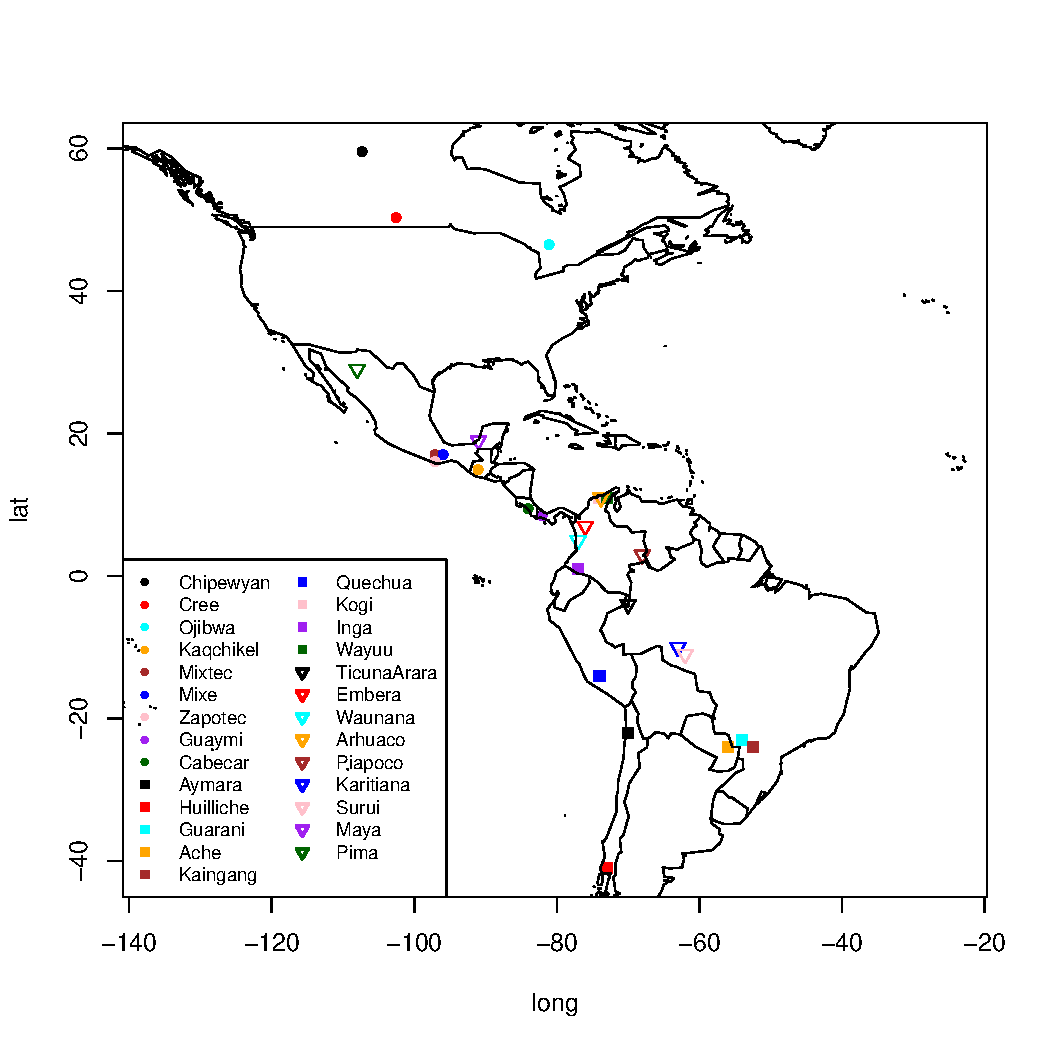
\includegraphics[scale=0.8]{figures/map.pdf}
		\caption{Répartition des populations autochtones sur le continent américain}
		\label{fig:map}
	\end{center}
\end{figure}
La question intéressante que nous nous posons est la suivante : un groupe
ethnique a t-il des caractéristiques propres et distinctives des autres
groupes ? Pour cela on peut retourner le problème en essayant de prédire des
quantités concernant les individus
en se basant seulement sur leurs ADN. \vspace{2mm}\\
Notre but est donc de construire un classificateur permettant d'associer un individu
à une population en fonction de ses 5709 marqueurs génétiques. Malheureusement
certaines populations présentent des effectifs très faibles. Par exemple, nous
ne disposons que de 7 individus de la population \textit{Kaingang} et de 10
individus pour la population \textit{Guarani}. Effectuer une classification
avec de si faibles effectifs ne seraient pas très pertinents.\vspace{2mm}

\begin{lstlisting}
	table(NAm2$Pop)
	##
	## Ache     Arhuaco      Aymara     Cabecar   Chipewyan        Cree      Embera 
	## 19          17          18          20          29          18          11 
	## Guarani      Guaymi   Huilliche        Inga    Kaingang   Kaqchikel   Karitiana 
	## 10          18          20          17           7          12          24 
	## Kogi        Maya        Mixe      Mixtec      Ojibwa     Piapoco        Pima 
	## 17          25          20          20          20          13          25 
	## Quechua       Surui TicunaArara     Waunana       Wayuu     Zapotec 
	## 20          21          17          20          17          19 
\end{lstlisting}
Pour palier ce problème, nous décidons alors d'effectuer la classification par
pays c'est à dire qu'un individu sera associé à un pays selon ses marqueurs
génétiques.  
\vspace{2mm}
\begin{lstlisting}
	table(NAm2$Country)
	## Brazil    Canada     Chile  Colombia CostaRica Guatemala    Mexico    Panama 
	## 62        67        38       129        20        12       109        18 
	## Paraguay      Peru 
	## 19             20 
\end{lstlisting}
Étudier ce problème de classification est mieux car d'une part le plus faible
effectif dans une classe est 12 ; ce qui est reste faible mais supérieur au cas
précédent. D'autre part le nombre de classes $K$ diminue. En effet, dans la
classification par pays, nous avions 27 classes tandis qu'ici nous n'en avons
plus que 10. Des méthodes telles que la régression logistique se comporte mieux
lorsque $K$ n'est pas très grand.\vspace{3mm}\\
La principale difficulté dans nos données provient du très grand nombre de variables explicatives. En effet nous sommes dans une situation où le nombre d'observations $n = 494$ est très petit par rapport au nombre de prédicteurs $p=5709$.\\
Dans ce présent travail, nous allons appliquer différentes méthodes à nos données pour ensuite en retenir la meilleure.
\section{Méthodes basées sur la réduction de dimension}
Dans un contexte de classification, la régression logistique apparaît comme un premier choix. Cependant $n$ étant très petit devant $p$, nous ne pouvons pas l'appliquer directement. Notre idée consiste donc à d'abord réduire la dimension en effectuant une analyse en composantes principales. Ensuite nous appliquons la régression logistique en utilisant quelques composantes comme variables indépendantes. Cette technique s'inspire essentiellement de la régression en composantes principales (PCR).\vspace{2mm}\\
Pour toute la suite, nous divisons notre jeu de données en un ensemble d'apprentissage et un ensemble test. En raison de notre faible nombre d'observations, notre ensemble de test ne contient que 94 observations.\vspace{2mm}
\begin{lstlisting}
	# lecture du jeu de données
	NAm2 = read.table("NAm2.txt", header = T)
	# séparation des donnees
	set.seed(12345)
	train = sample(1:nrow(NAm2), 400)
\end{lstlisting}
\subsection{Analyse en composantes principales}
Nous effectuons une analyse en composantes principales sur les 5709 variables explicatives. Les variables génétiques étant binaires, il n'est pas nécessaire ici qu'elles soient réduites. Le code ci-contre permet d'effectuer l'analyse. \vspace{2mm}
\begin{lstlisting}
	pca = prcomp(NAm2[train,-c(1:8)])
	pvar = ((pca$sdev/sum(pca$sdev))**2)*100
	par(mfrow=c(1,2))
	plot(1:length(pvar), pvar, type="p", col="blue", xlab="composantes",
			ylab="pourcentage de variance expliquée", cex=0.5)
	plot(1:length(pvar), cumsum(pvar), type="l", lwd=1.5, col="blue", xlab="composantes", ylab="pourcentage de variance cumulee")
	par(mfrow=c(1,1))
\end{lstlisting}
\begin{figure}[h!]
	\begin{center}
		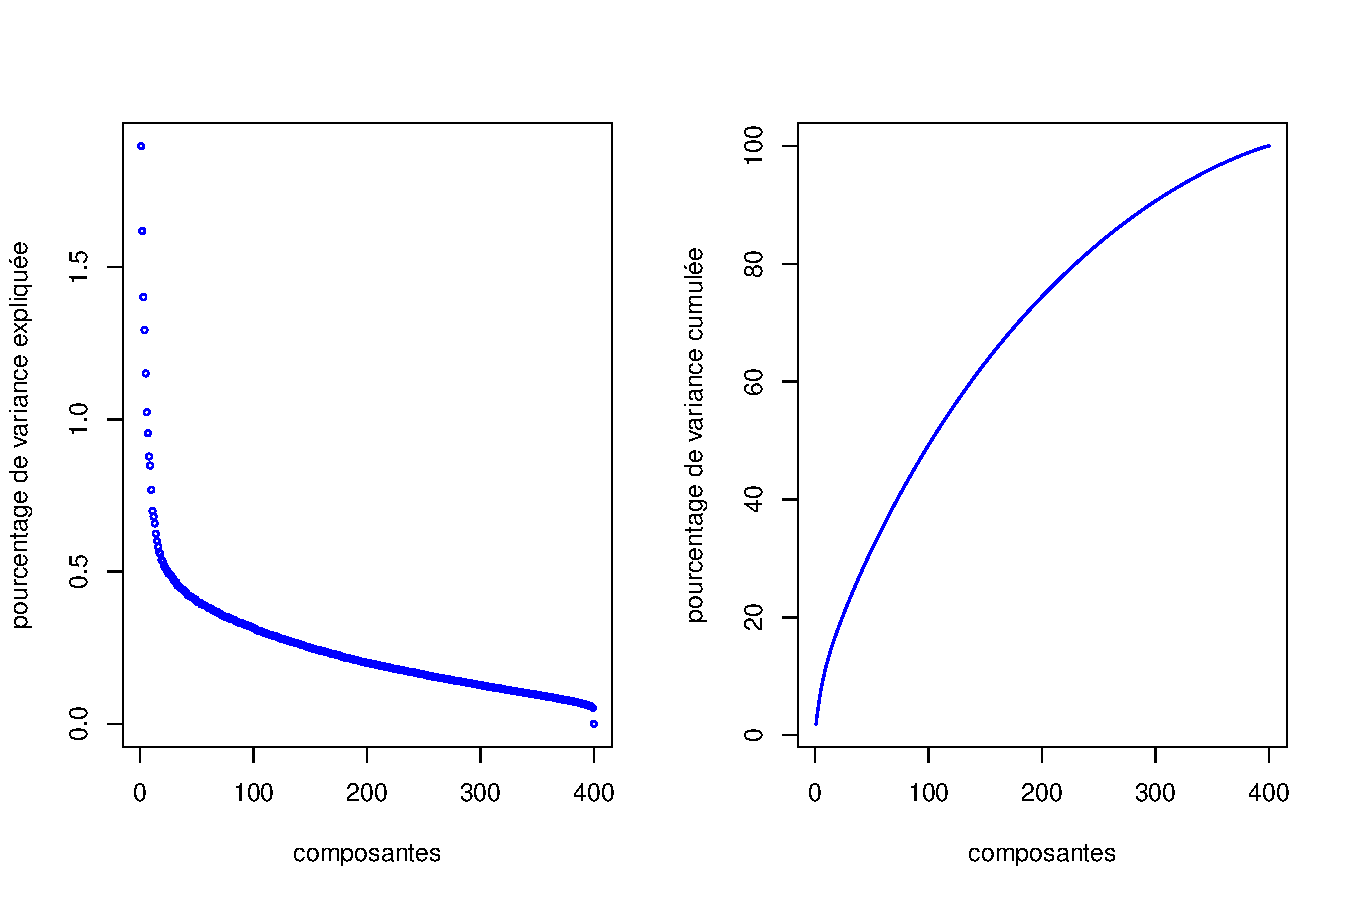
\includegraphics[scale=0.7]{figures/pca_plot.pdf}
		\caption{Pourcentage de variance expliquée pour chaque composante à gauche et le pourcentage cumulé à droite}
		\label{fig:acp_plot}
	\end{center}
\end{figure}
Nous obtenons 400 composantes principales. La figure \ref{fig:acp_plot}
représente le pourcentage de variance expliquée pour chaque composante à gauche
et le pourcentage cumulé à droite. On peut noter que les 100 premières
composantes expliquent environ 49\% de la variance et les 200 premières un peu
moins de 75.  

\noindent L'ACP est intéressante car elle a un aspect 'visuel', on peut projeter par
exemple les données sur deux composantes principales et afficher les données
dans le plan. On prend par exemple les composantes 3 et 6 qui ont un beau
rendu. Effectivement sur la figure \ref{fig:acp_pc36}, on voit deux, voire trois
groupes se dégager, les \textit{Surui}, les \textit{Pima} et les \textit{Arhuaco}. Cela confirme l'intérêt
de se baser sur les composantes principales pour analyser nos données.
\begin{figure}[h!]
	\begin{center}
		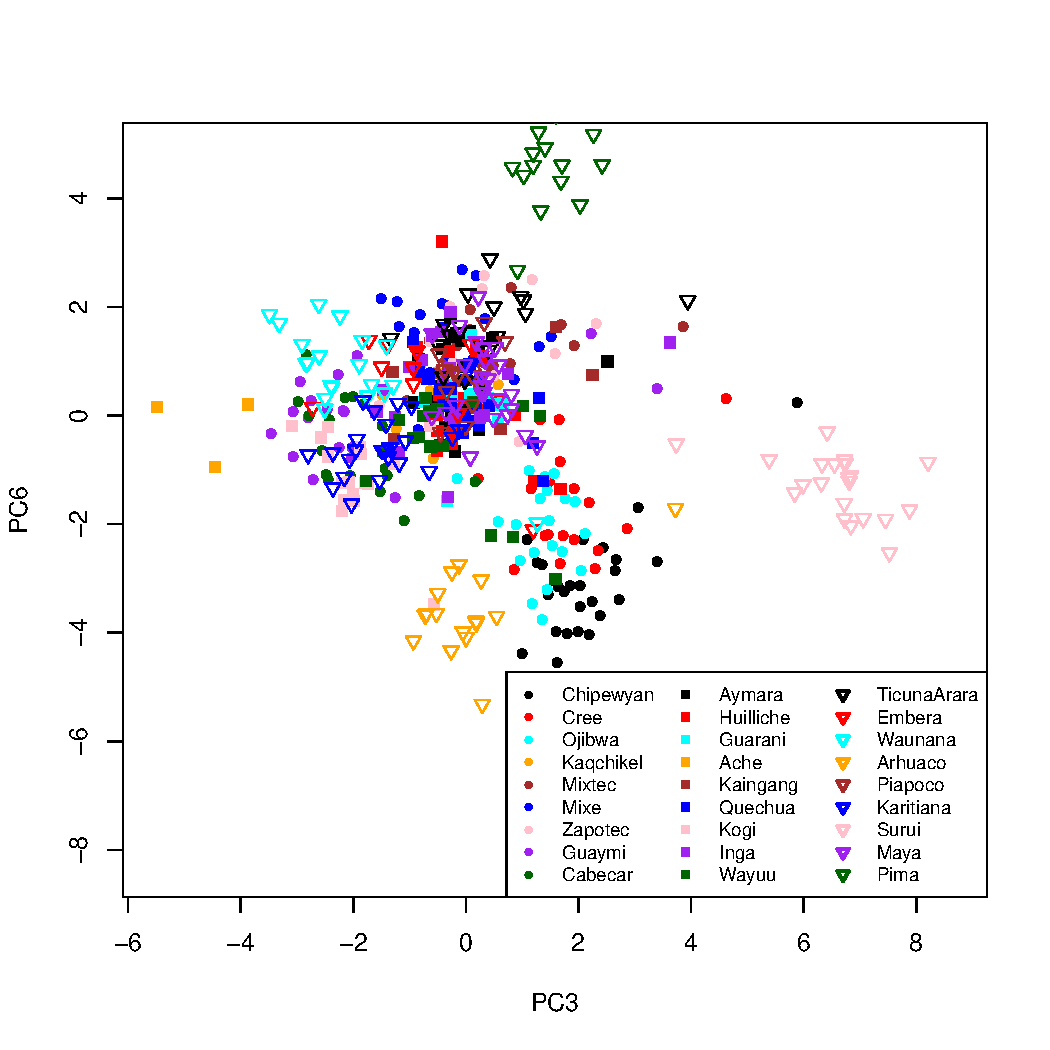
\includegraphics[scale=0.7]{figures/pc36.pdf}
		\caption{Projection des données sur les composantes principales 3 et 6}
		\label{fig:acp_pc36}
	\end{center}
\end{figure}

Voici le code utilisé pour générer la figure \ref{fig:acp_pc36}.
\begin{lstlisting}
	comps=c(3,6)
	plot(pca$x[,comps],col="white")
	for (i in 1:length(names)) {
		print(names[i])
		lines(pca$x[which(NAm2[,3]==names[i]),comps],type="p",col=colPalette[i],pch=pch[i])
	}
	legend("bottomright",legend=names,col=colPalette,lty=-1,pch=pch,cex=.75,ncol=3,lwd=2, bg="white")
\end{lstlisting}
Maintenant que nous avons les composantes principales, nous
pouvons effectuer la régression logistique.
\subsection{Régression logistique} 
Pour effectuer la régression logistique, nous devons d'abord choisir le nombre
de composantes principales. Nous pourrions appliquer la méthode du \og coude
\fg  pour choisir le nombre de composantes optimal mais nous préférons utiliser
la validation croisée. En effet, nous allons considérer des nombres différents
de composantes et calculer le taux d'erreur en utilisant un \og 10-folds\fg.
Nous choisissons alors le nombre de composantes pour lequel ce taux d'erreur
sera minimal.\\
Notons que pour faire la régression logistique nous utilisons la fonction
\textbf{multiom()} du package \textbf{nnet}.\vspace{2mm}

\begin{lstlisting}
	# La fonction cv_error calcule le taux d'erreur par validation croisée pour un 
	# nombre de composantes donne
	cv_error <- function(idx, ncomp, method) {
		nfolds = 40
		err = numeric(10)
		for (k in 0:9) {
			sub = idx[(nfolds*k+1):(nfolds*(k+1))]
			gen = data.frame(Country=NAm2$Country[train], pca$x[,1:ncomp])
			if(method == "logistic") {
				fit = multinom(Country~., data=gen, MaxNWts=20000, subset=-sub, trace=F)
				preds = predict(fit, newdata = gen[sub,], type="class")
			} else if(method=="lda") {
				fit = lda(Country~.,data=gen, subset=-sub)
				preds = predict(fit, newdata = gen[sub,], type="response")$class
			} else {
				return("NA")
			}
				err[k+1] = mean(gen$Country[sub]!=preds)
			}
			mean(err)
	}
\end{lstlisting}
\begin{lstlisting}
	require(nnet)
	ncomp = unique(c(seq(20,100,5), seq(100, 400, 20)))
	miscl = numeric(length(ncomp))
	set.seed(12345)
	idx = sample(1:400)
	j = 1
	for (i in ncomp) {
		cat(j,"/", 32, "\n")
		miscl[j] = cv_error(idx, i, "logistic")
		j = j+1
	}
	plot(ncomp, miscl, type='o', cex=0.6, col="blue", ylab = "taux erreur",
			xlab="nombre de composantes")
	ncomp_opt = ncomp[which.min(miscl)]
	## [1] 75
\end{lstlisting}
\begin{figure}[h!]
	\begin{center}
		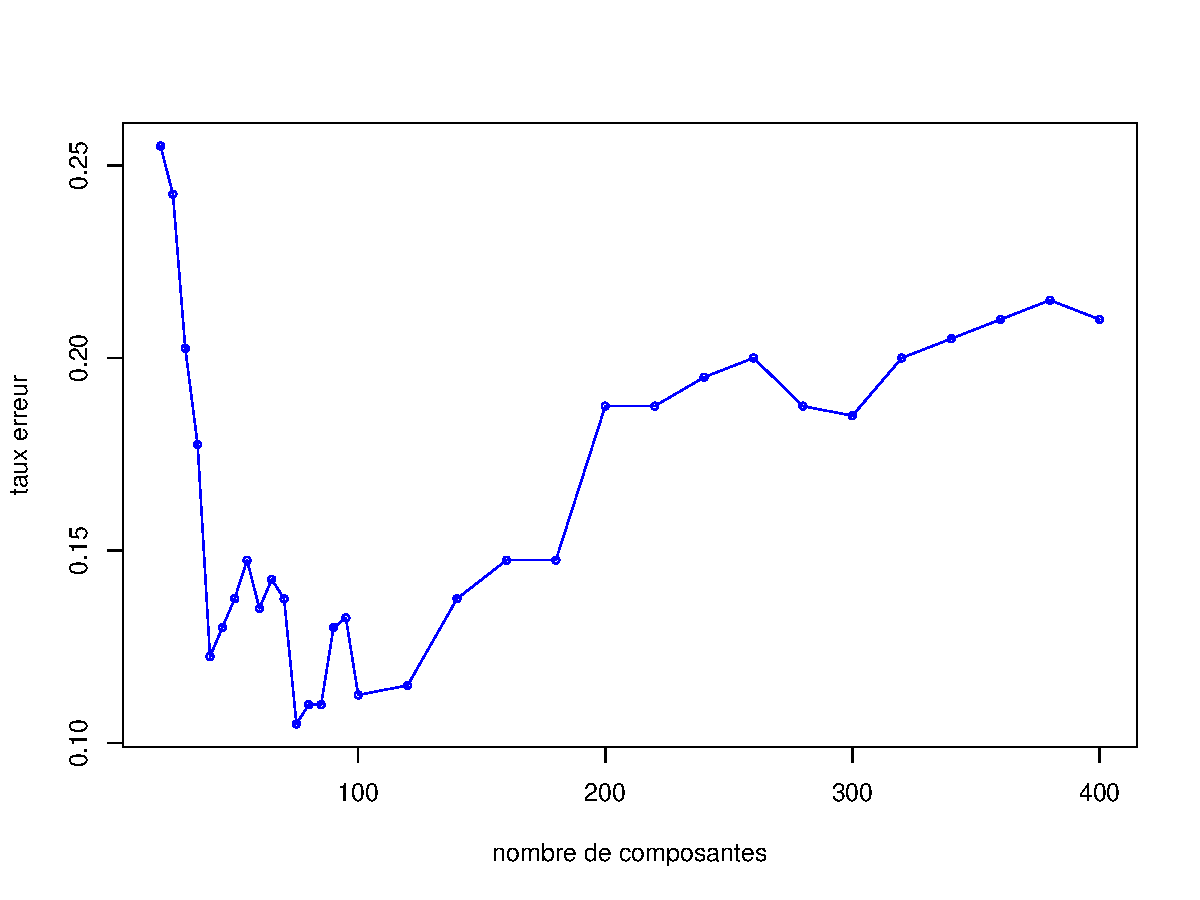
\includegraphics[scale=0.5]{figures/nopt_log.pdf}
		\caption{Taux d'erreur en fonction du nombre de composantes pour la régression logistique}
		\label{fig:nopt_log}
	\end{center}
\end{figure}
La figure \ref{fig:nopt_log} représente le taux d'erreur en fonction du nombre de composantes. On voit que celui-ci diminue dans un premier temps mais commence à remonter assez tôt à partir de 100 composantes. Le minimum est atteint pour 75 composantes soit 40.89\% de variance expliquée. Naïvement, on aurait pu penser que prendre 300 composantes aurait été un meilleur choix puisqu'elles expliquent plus de 80\% de la variance.\vspace{3mm}\\
Une fois le nombre de composantes principales déterminé, nous pouvons appliquer notre classificateur sur notre ensemble test. D'abord il faut que nous projetons les données de l'ensemble test sur les axes de l'ACP.
\begin{lstlisting}
	# projetcion des donnees test sur les axes de l ACP
	test_data = scale(NAm2[-train,-c(1:8)], pca$center, pca$scale) %*% pca$rotation
	test.log = as.data.frame(test_data[,1:ncomp_opt])
	
	# ajustemrnt du modèle
	gen_log = data.frame(Country=NAm2$Country[train], pca$x[,1:ncomp_opt])
	fit.log = multinom(Country~., data=gen_log, MaxNWts=20000, trace=F)
	
	# prediction des donnees
	preds.log = predict(fit.log, newdata = test.log, type="class")
	mean(NAm2$Country[-train]!=preds.log)
	## [1] 0.106383
\end{lstlisting}
Nous trouvons un taux d'erreur égale\vspace{-5mm} \[Err_{ACP}^{log} = 0.106\] soit 10 personnes mal classées sur 94. Quand on regarde plus en détails les erreurs, on voit qu'un seul individu de \textbf{Peru} a été bien classé sur les cinq présents. Aussi le seul guatémaltèque a été mal classé. On peut noter que l'ensemble d'apprentissage ne contenaient que 10 individus dans ces deux classes.\vspace{2mm}
\begin{lstlisting}
	table(NAm2$Country[-train], preds.log)
	## 			Brazil Canada Chile Colombia CostaRica Guatemala Mexico Panama Paraguay Peru
	## Brazil     9      0     0        1         0         0      1      0        0          0
	## Canada     0     15     0        0         0         0      0      0        0          0
	## Chile      0      0     7        0         0         0      0      0        0          0
	## Colombia   0      1     0       21         0         0      1      0        0          0
	## CostaRica  0      0     0        0         3         0      0      0        0          0
	## Guatemala  0      0     0        1         0         0      0      0        0          0
	## Mexico     0      0     0        1         0         0     22      0        0          0
	## Panama     0      0     0        0         0         0      0      2        0          0
	## Paraguay   0      0     0        0         0         0      0      0        4          0
	## Peru       1      0     1        2         0         0      0      0        0          1
\end{lstlisting}
\subsection{Analyse discriminante linéaire}
Un autre classificateur très populaire est celui de l'analyse discriminante linéaire. Une hypothèse de normalité au sein des variables explicatives est tout à fait plausible dans ce contexte. Nous avons d'abord essayer d'appliquer la méthode directement sur les données mais celle-ci a échoué. En effet même si théoriquement elle peut marcher sur ces données, l'inversion de la matrice de covariance $\Sigma$ est très instable numériquement.\\
Nous avons donc décider comme pour la régression logistique d'appliquer l'analyse sur les composantes principales. Ici aussi un choix du nombre de composantes est fait par validation croisée. Le code R ci-contre permet d'effectuer cette sélection.\vspace{2mm}
\begin{lstlisting}
	require(MASS)
	ncomp_lda = seq(20,340,5)
	misc = numeric(length(ncomp_lda))
	set.seed(12345)
	j=1
	for (i in ncomp_lda) {
		cat(j,"/", 65, "\n")
		misc[j] = cv_error(idx, i, "lda")
		j = j+1
	}
	plot(ncomp_lda, misc, type='o', cex=0.6, col="blue", ylab = "taux erreur",
			xlab="nombre de composantes")
	nopt_lda = ncomp_lda[which.min(misc)]
	## [1] 135
\end{lstlisting}

\begin{figure}[h!]
	\begin{center}
		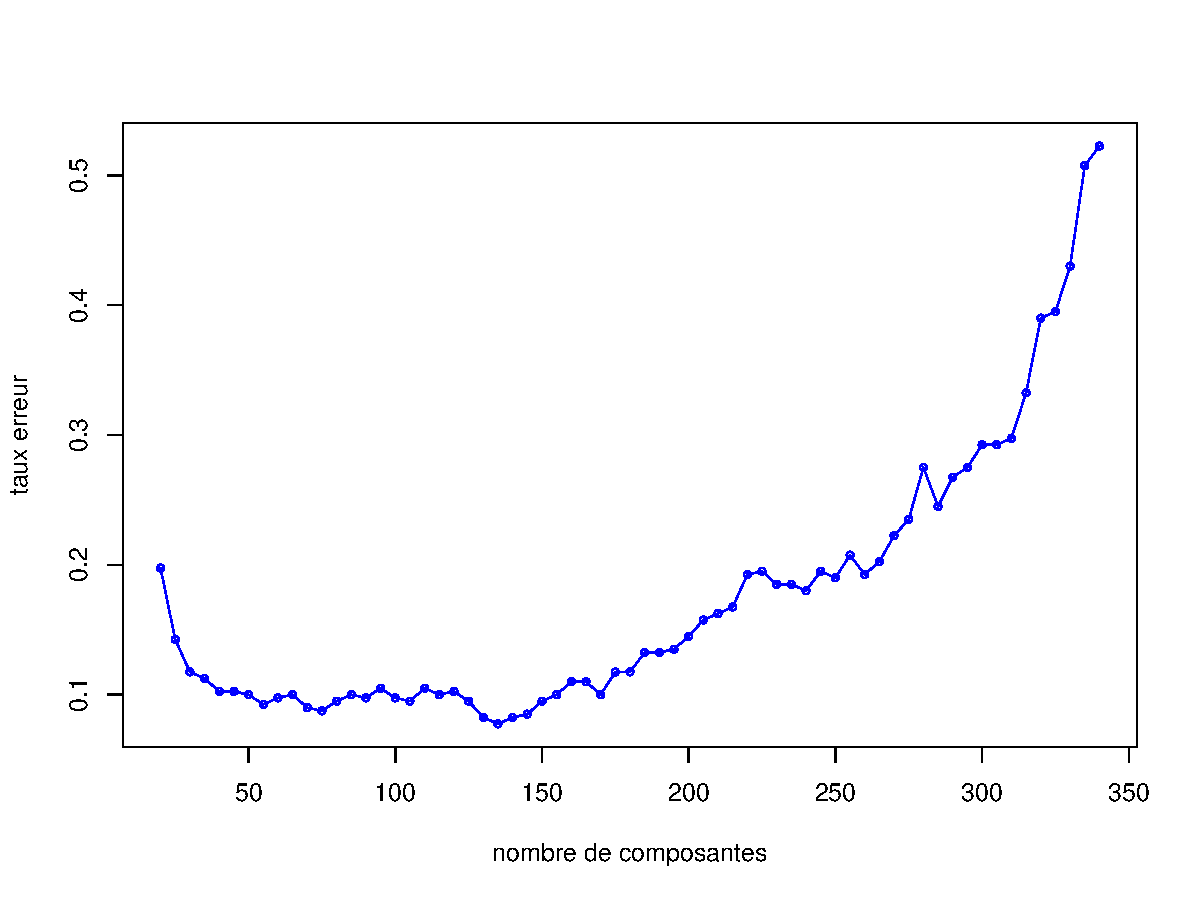
\includegraphics[scale=0.5]{figures/nopt_lda.pdf}
		\caption{Taux d'erreur en fonction du nombre de composantes pour l'analyse discriminante linéaire}
		\label{fig:nopt_lda}
	\end{center}
\end{figure}
\noindent La figure \ref{fig:nopt_lda} représente le taux d'erreur en fonction du nombre de composantes. Ce taux est minimal pour 135 composantes. On sélectionne environ deux fois plus de composantes avec cette méthode. Ce qui montre que le nombre de composantes à choisir est propre à chaque méthode. Nous calculons donc le taux d'erreur test avec 135 composantes.\vspace{2mm}
\begin{lstlisting}
	# donnees pour la LDA
	gen_lda = data.frame(Country=NAm2$Country[train], pca$x[,1:nopt_lda])
	# ajustement
	fit.lda = lda(Country~.,data=gen_lda)
	test.lda = as.data.frame(test_data[,1:nopt_lda])
	preds.lda = predict(fit.lda, newdata = test.lda, type="response")$class
	mean(NAm2$Country[-train] != preds.lda)
	## 0.09574468
\end{lstlisting}
On obtient un taux d'erreur \vspace{-3mm}\[Err_{ACP}^{LDA} = 0.096\]
L'analyse linéaire discriminante classe correctement un individu de plus que la régression logistique. En effet elle classe correctement un individu de \textit{Mexico}. Les deux méthodes classent mal deux habitants de \textit{Brazil} mais se trompent différemment pour l'un des deux. Le reste est identique. \vspace{4mm}\\
Nous avons essayé d'appliquer l'analyse discriminante quadratique en suivant le même schéma mais celle-ci a échoué car une classe ne contenait pas assez d'effectifs.

\section{Régression logistique régularisée}
Une façon de contourner le problème de dimension ($n\ll p$) consiste à utiliser
des méthodes de régularisation qui consistent essentiellement à ajouter une
pénalité dans la fonction objective que nous cherchons à minimiser (ou
maximiser) dans nos algorithmes. Ainsi dans cette partie, nous utilisons
toujours la régression logistique mais en appliquant une régularisation. Nous
considérons les régularisations Lasso et Ridge.

\subsection{Régularisation Ridge}
Comme dans le cas de la régression linéaire, nous utilisons le package \textbf{glmnet}. Nous choisissons la valeur optimale de $\lambda$ par validation croisée.
\begin{lstlisting}
	require(glmnet)
	x = model.matrix(Country~., data=NAm2[train, -c(1:3,5:8)])[,-1]
	set.seed(12345)
	fit.log_ridge = glmnet(x=x, y=NAm2$Country[train], alpha = 0, family="multinomial")
	plot(fit.log_ridge, xvar = "lambda")
\end{lstlisting}
\begin{figure}[h!]
	\begin{center}
		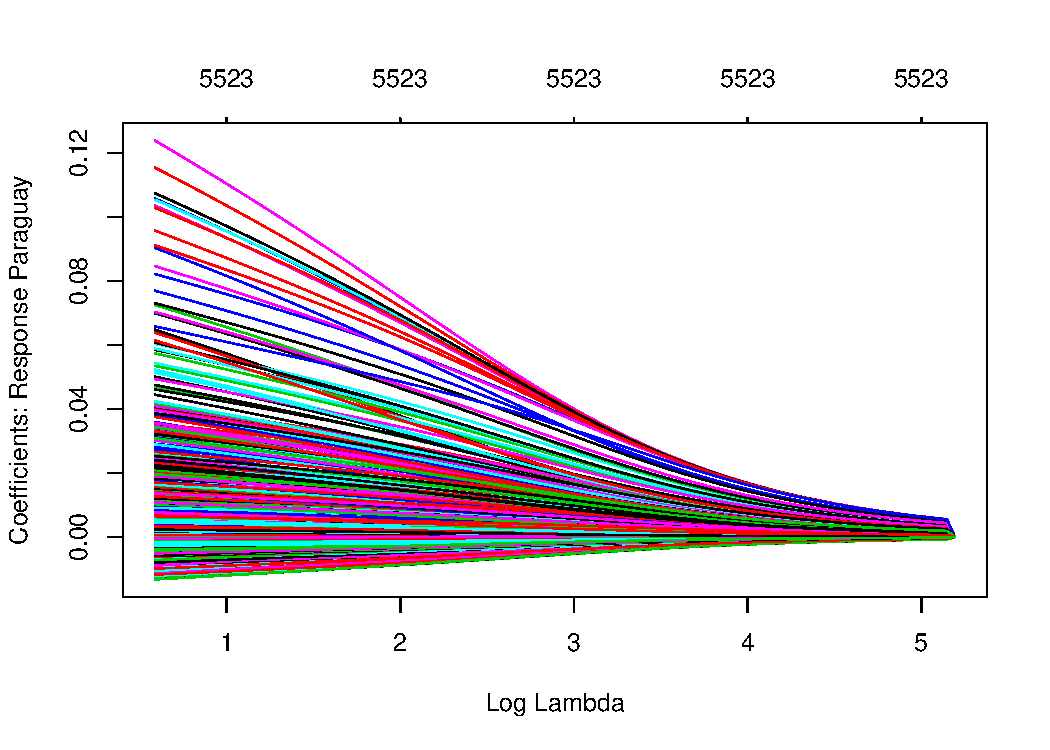
\includegraphics[scale=0.5]{figures/coef_ridge.pdf}
		\caption{Évolution des coefficients de la régression logistique pour la classe \textbf{Paraguay} en fonction du $\log(\lambda)$}
		\label{fig:r_lambda}
	\end{center}
\end{figure}
La figure \ref{fig:r_lambda} représente l'évolution des coefficients de la
régression logistique pour la classe \textbf{Paraguay} en fonction du
logarithme de $\lambda$. On voit bien l'effet du rétrécissement des
coefficients qui tendent vers 0 pour de grandes valeurs de $\lambda$.\\
Le graphique de gauche sur la figure \ref{fig:r_lopt} montre l'évolution du
taux d'erreur en fonction de $\lambda$. Ce graphique suggère que la valeur
optimale de $\lambda$ se trouve dans les faibles valeurs. Nous changeons alors
notre grille de recherche et obtenons le graphique de droite sur la figure
\ref{fig:r_lopt}. Plusieurs valeurs donnent un taux d'erreur minimal (figure
\ref{fig:zoom_r} ); on choisit alors $\lambda^* = 0.001$.\vspace{2mm}

\begin{figure}[h!]
	\begin{center}
		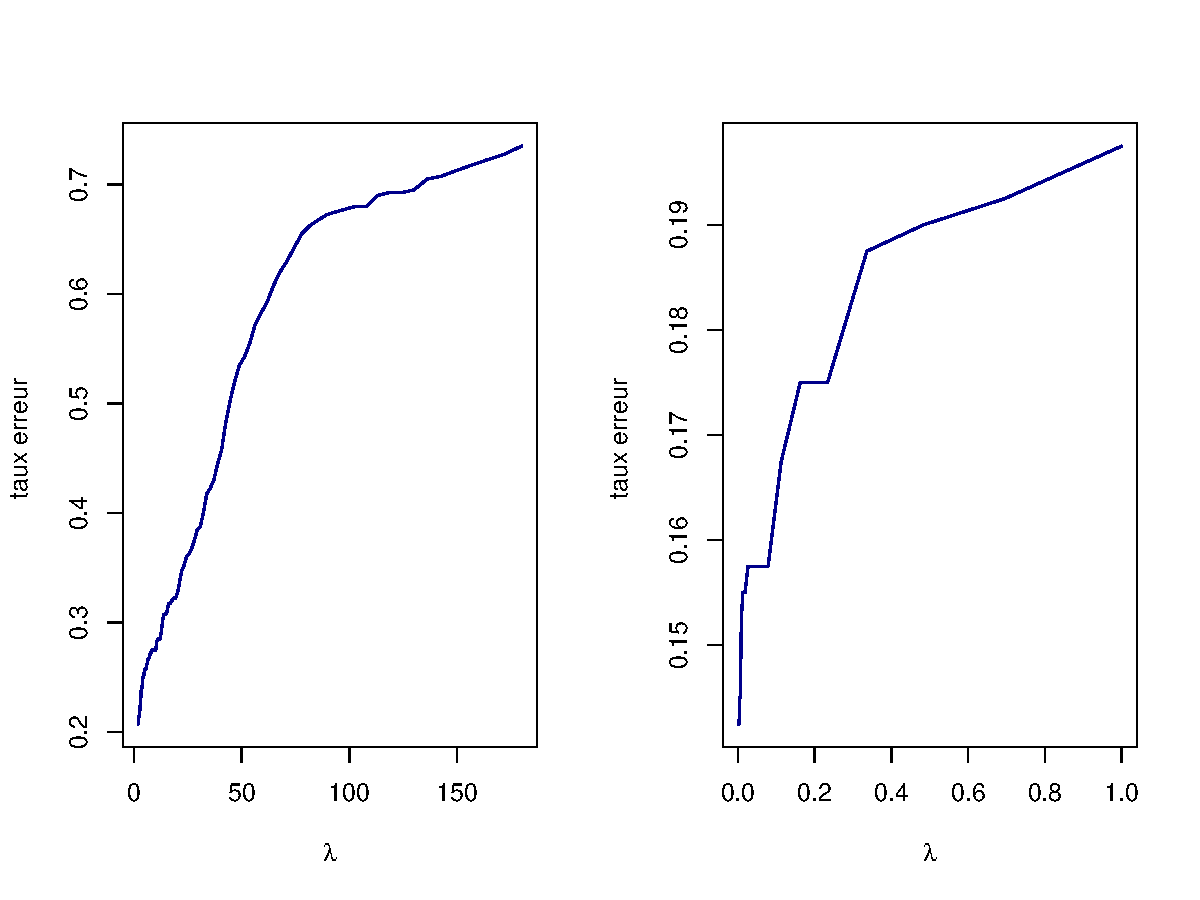
\includegraphics[scale=0.7]{figures/r_lopt.pdf}
		\caption{Taux d'erreur en fonction de $\lambda$ pour la régression Ridge.}
		\label{fig:r_lopt}
	\end{center}
\end{figure}
\begin{figure}[h!]
	\begin{center}
		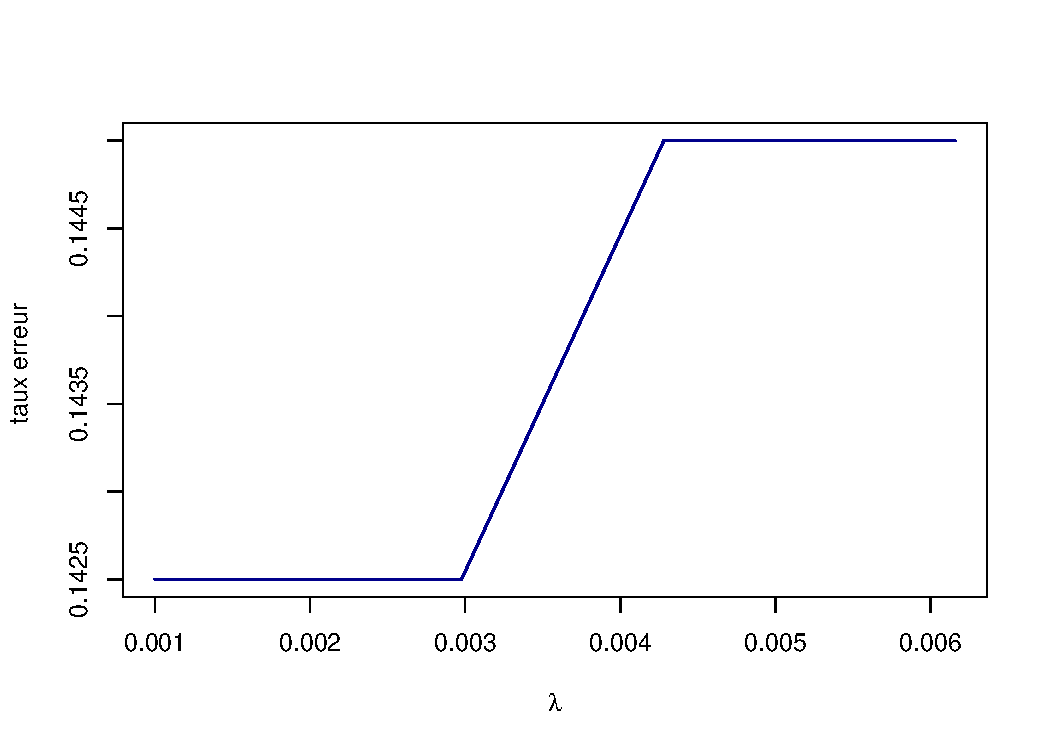
\includegraphics[scale=0.5]{figures/zoom_r_lopt.pdf}
		\caption{Zoom sur les petites valeurs du graphique de droite de la figure \ref{fig:r_lopt}}
		\label{fig:zoom_r}
	\end{center}
\end{figure}
\begin{lstlisting}
	set.seed(12345)
	cv.ridge = cv.glmnet(x=x, y=NAm2$Country[train], alpha=0, family="multinomial",
							type.measure = "class")
	par(mfrow=c(1,2))
	plot(cv.ridge$lambda, cv.ridge$cvm, type='l', xlab=expression(lambda),
			ylab = "taux erreur ", lwd = 1.5, col="darkblue")
	# on ajuste la grille de recherche		
	grid = 10^seq (0, -3, length =20)
	set.seed(12345)
	cv.ridge = cv.glmnet(x=x, y=NAm2$Country[train], alpha=0, family="multinomial",
										type.measure = "class", lambda = grid)
	plot(cv.ridge$lambda, cv.ridge$cvm, type='l', xlab=expression(lambda),
				ylab = "taux erreur ", lwd = 1.5, col="darkblue")
	par(mfrow=c(1,1))
\end{lstlisting}
On calcule maintenant le taux d'erreur sur l'ensemble test. \vspace{2mm}
\begin{lstlisting}
	newx = model.matrix(Country~., data=NAm2[-train, -c(1:3,5:8)])[,-1]
	preds.ridge = predict.cv.glmnet(cv.ridge, newx=newx, s=0.001, type = "class")
	mean(NAm2$Country[-train] != preds.ridge)
	## [1] 0.05319149
\end{lstlisting}
On obtient un taux d'erreur plus petit que celui des deux méthodes précédentes.\vspace{-3mm} \[Err_{Ridge}^{log} = 0.053\vspace{-4mm}\]
Nous classons correctement 89 individus sur 94. Un des deux brésiliens a été bien classé. Aussi un seul péruvien sur cinq est correctement classé. On notera que ce classificateur ne se trompe pas de la même manière que les deux autres sur les péruviens. \vspace{2mm}
\begin{lstlisting}
	table(NAm2$Country[-train], preds.ridge)
	## 			Brazil Canada Chile Colombia CostaRica Guatemala Mexico Panama Paraguay Peru
	## Brazil    10      0     0        1         0         0      0      0        0        0
	## Canada     0     15     0        0         0         0      0      0        0        0
	## Chile      0      0     7        0         0         0      0      0        0        0
	## Colombia   0      0     0       23         0         0      0      0        0        0
	## CostaRica  0      0     0        0         3         0      0      0        0        0
	## Guatemala  0      0     0        0         0         1      0      0        0        0
	## Mexico     0      0     0        0         0         0     23      0        0        0
	## Panama     0      0     0        0         0         0      0      2        0        0
	## Paraguay   0      0     0        0         0         0      0      0        4        0
	## Peru       0      1     0        3         0         0      0      0        0        1
\end{lstlisting}
\subsection{Régularisation Lasso}
Le code R ci-contre permet d'effectuer l'ajustement.
\begin{lstlisting}
	set.seed(12345)
	cv.lasso = cv.glmnet(x=x, y=NAm2$Country[train], family="multinomial",
	                     type.measure = "class")
	par(mfrow=c(1,2))
	plot(cv.lasso$lambda, cv.lasso$cvm, type='l', xlab=expression(lambda),
	     ylab = "taux erreur ", lwd = 1.5, col="darkblue")
	plot(cv.lasso$lambda[cv.lasso$cvm<0.3], cv.lasso$cvm[cv.lasso$cvm<0.3], type='l', xlab=expression(lambda),
	     ylab = "taux erreur ", lwd = 1.5, col="darkblue")
	par(mfrow=c(1,2))
\end{lstlisting}
\begin{figure}[h!]
	\begin{center}
		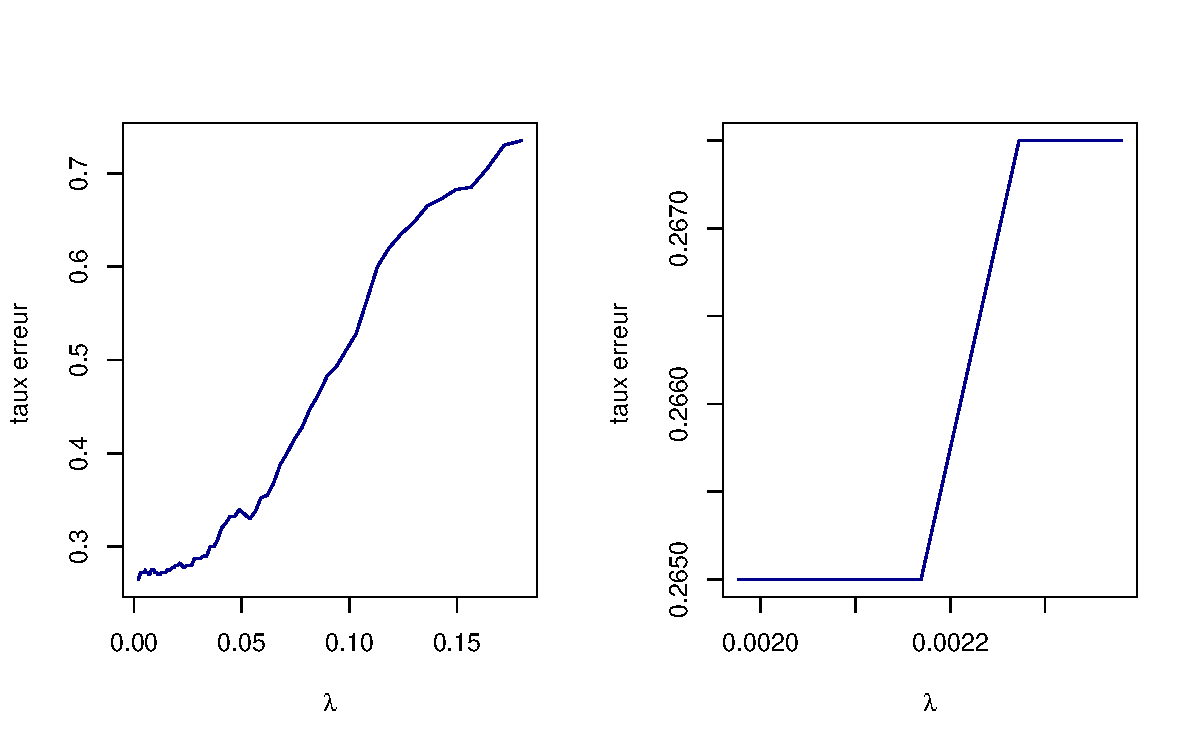
\includegraphics[scale=0.7]{figures/l_opt.pdf}
		\caption{Taux d'erreur en fonction de $\lambda$ pour la régression Lasso ; la figure de  droite fait un zoom sur les petites valeurs}
		\label{fig:l_opt}
	\end{center}
\end{figure}
La figure \ref{fig:l_opt} représente l'évolution du taux d'erreur en fonction
de $\lambda$. Le graphique de droite fait un zoom sur les petites valeurs. Ici
aussi on voit qu'une petite valeur de $\lambda$ est optimale. On choisit donc
$\lambda_{lasso}^* = 0.002$.\\
Nous calculons le taux d'erreur sur l'ensemble de test.

\begin{lstlisting}
	preds.lasso = predict.cv.glmnet(cv.lasso, newx=newx, s=0.002, type = "class")
	mean(NAm2$Country[-train] != preds.lasso)
	## [1] 0.1382979
\end{lstlisting}
Nous obtenons un taux d'erreur plus élevé que toutes celui des trois méthodes
précédentes. En effet nous ne classons correctement que 81 individus. On peut
remarquer qu'aucun individu de\textit{Panama} n'a été prédit alors qu'il y'en avait deux. Par contre cette
méthode fait mieux que les précédentes sur les individus de \textit{Péru}
puisqu'elle en classe correctement~2.\vspace{3mm}\\
On pourrait donc penser à utiliser une régularisation de type \og elastic net \fg pour prendre en compte les deux pénalités Lasso et Ridge puisque Lasso semble mieux prédire les individus de \textit{Péru}. Cette technique n'a toutefois pas été testé dans ce projet.
\section{Méthodes non paramétriques}
\subsection{K plus proches voisins}
Une autre méthode populaire de classification est la méthode des plus proches
voisins. Cette méthode utilise le concept de distance. Elle est
pertinente car on voudrait que les individus ayant des ADN proches (en terme
de la distance utilisée par KNN) soit de la même population ou du même pays. \\
Aussi les méthodes utilisées précédemment supposent que nos données
sont linéairement séparables. La méthode KNN quant à elle peut produire un
classificateur non linéaire.\vspace{3mm}\\
Ici une réduction des données n'est pas nécessaire. Nous utilisons directement
nos données et choisissons le $K$ optimal par validation croisée. Nous
faisons varier $K$ de 2 à 30. Le code R ci-contre permet d'effectuer cette
sélection.\vspace{2mm}
\begin{lstlisting}
	require(class)
	nfolds = 40
	K = 2:30
	err = numeric(length(K))
	set.seed(12345)
	for (i in K) {
		tmp = 0
		cat(i-1,"/",29, "\n")
		for (k in 0:9) {
			sub = (nfolds*k+1):(nfolds*(k+1))
			fit = knn(train=NAm2[train[-sub], -(1:8)], test=NAm2[train[sub], -(1:8)],
						cl=NAm2$Country[train[-sub]], k=i)
			tmp = tmp + mean(NAm2$Country[train[sub]]!=fit)
		}
		err[i-1] = tmp/10
	}
	plot(K, err, type='o', col='blue', lwd=1.5, ylab="taux d'erreur")
\end{lstlisting}
\begin{figure}[h!]
	\begin{center}
		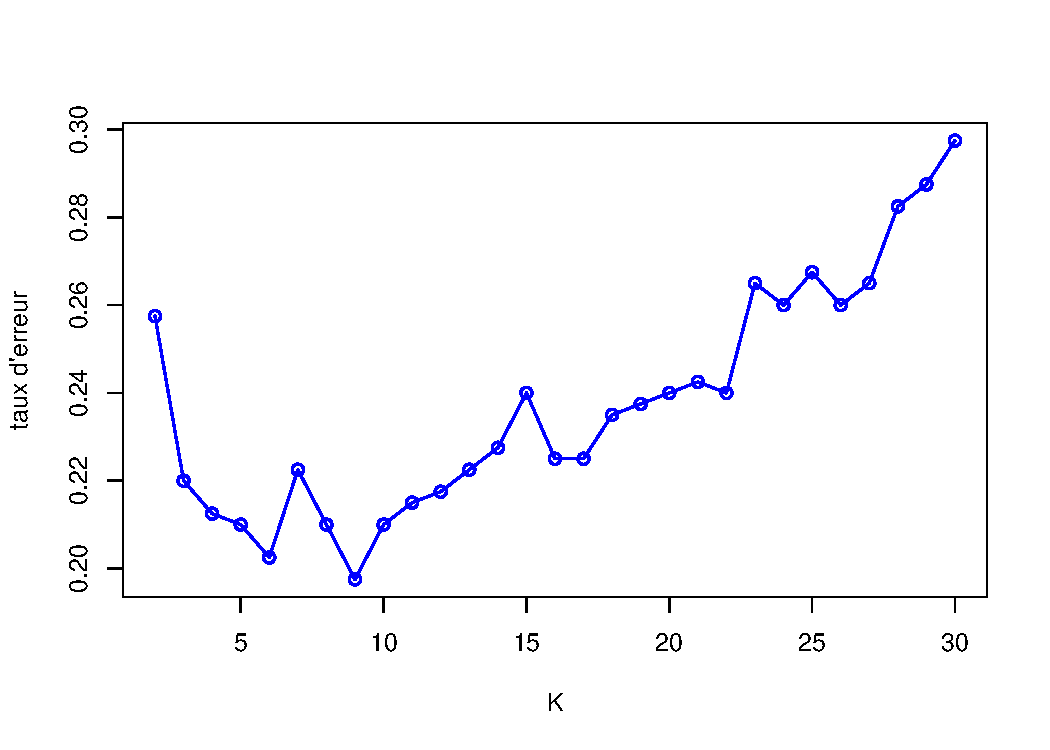
\includegraphics[scale=0.6]{figures/kopt.pdf}
		\caption{Taux d'erreur en fonction de $K$.}
		\label{fig:kopt}
	\end{center}
\end{figure}
La figure \ref{fig:kopt} représente l'évolution du taux d'erreur en fonction de $K$. Le taux d'erreur est minimal pour $K^* = 9$. Nous calculons maintenant le taux d'erreur sur l'ensemble test.\vspace{2mm}
\begin{lstlisting}
	preds.knn = knn(train=NAm2[train,-(1:8)], test = NAm2[-train, -(1:8)],
	                cl=NAm2$Country[train], k=kopt)
	mean(NAm2$Country[-train] != preds.knn)
	## [1] 0.1489362
\end{lstlisting}
Elle classe un individu moins bien que la régression logistique avec Lasso. Elle aussi ne classe correctement qu'un seul des cinq individus de \textit{Péru}.
\subsection{Arbres de décision}
La dernière classe de méthodes que nous considérons est celle basée sur les arbres de décision. Dans cette partie, nous appliquons un arbre de classification, du bagging et du random forests. Ces méthodes ne nécessitent pas une réduction de dimension ; elles s'appliquent directement aux données.
\subsubsection{Arbre de classification}
Le code ci-contre permet d'effectuer l'ajustement d'un arbre de classification. Notons que nous utilisons le package \textbf{rpart} plutôt que le package \textbf{tree}. En effet ce dernier ne marchait pas sur les données.\vspace{2mm}
\begin{lstlisting}
	require(rpart)
	set.seed(12345)
	fit.tree = rpart(Country~., data=NAm2[,-c(1:3,5:8)], subset = train, method ="class",
	                 control = rpart.control(minsplit = 5, maxdepth = 30))
	plot(fit.tree)
	text(fit.tree, cex=.5, pretty = 0)
\end{lstlisting}
\begin{figure}[h!]
	\begin{center}
		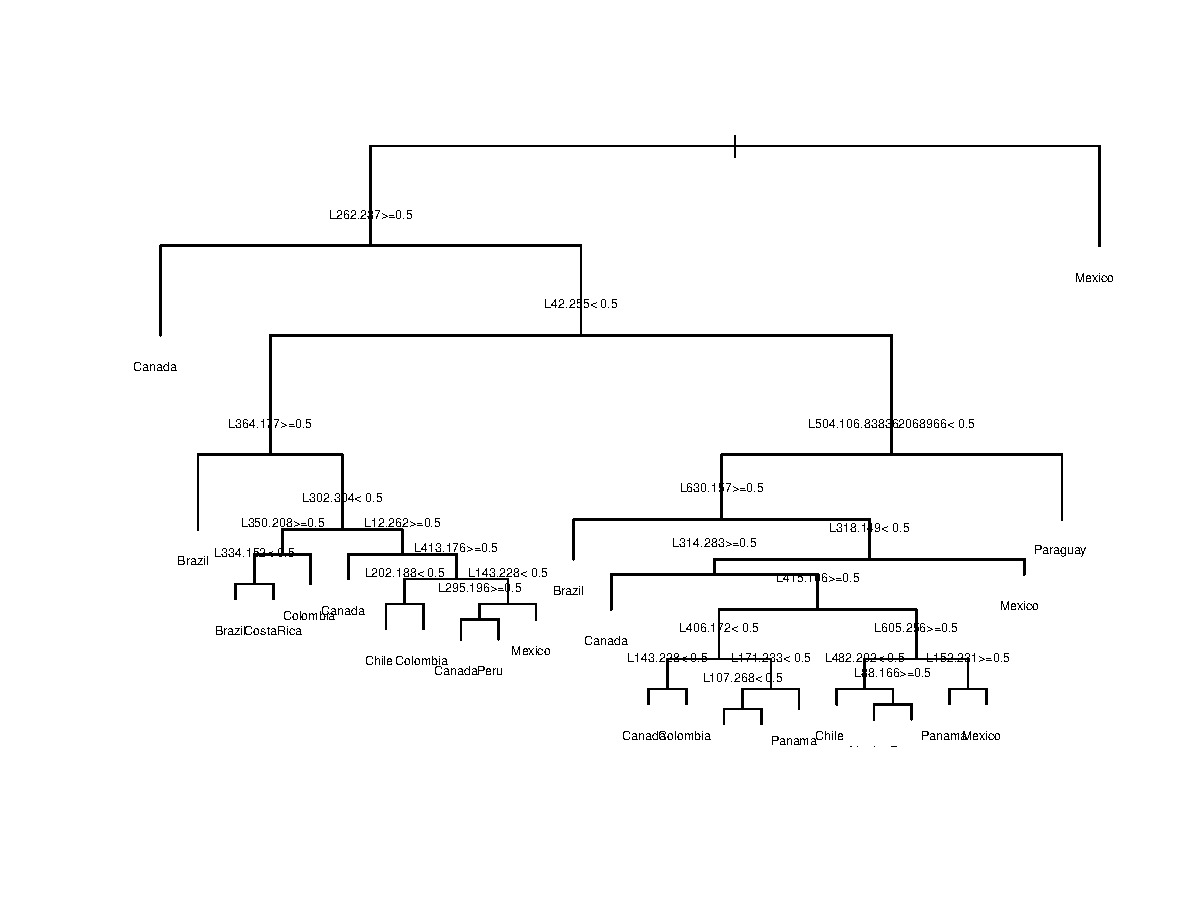
\includegraphics[scale=0.8]{figures/tree.pdf}
		\caption{Arbre de classification.}
		\label{fig:tree}
	\end{center}
\end{figure}
La figure \ref{fig:tree} représente l'arbre obtenu. On note que sur les 5709 variables disponibles seules 24 ont été utilisées pour construire l'arbre. Aussi on note que les classes \textit{Canada} et \textit{Mexico} sont identifiées très haut dans l'arbre. On retrouve les avantages d'interprétation des arbres.\\
Nous obtenons un taux d'erreur sur l'ensemble de test très élevé : \hspace{5mm}$Err_{tree} = 0.489$. Il est certes meilleur que le classificateur uniforme mais comparativement aux méthodes précédentes, il est très mauvais. \vspace{2mm}
\begin{lstlisting}
	preds.tree = predict(fit.tree, newdata = NAm2[-train,-c(1:3,5:8)], type = "class")
	mean(NAm2$Country[-train] != preds.tree)
	table(NAm2$Country[-train], preds.tree)
	## [1] 0.4893617
\end{lstlisting}
Une technique pour améliorer le modèle consiste à couper l'arbre plus tôt.\vspace{2mm}
\begin{lstlisting}
	prun = prune(fit.tree, cp = fit.tree$cptable[which.min(fit.tree$cptable[,"xerror"]),"CP"])
	plot(prun)
	text(prun, cex=.5, pretty = 0)
\end{lstlisting}
\begin{figure}[h!]
	\begin{center}
		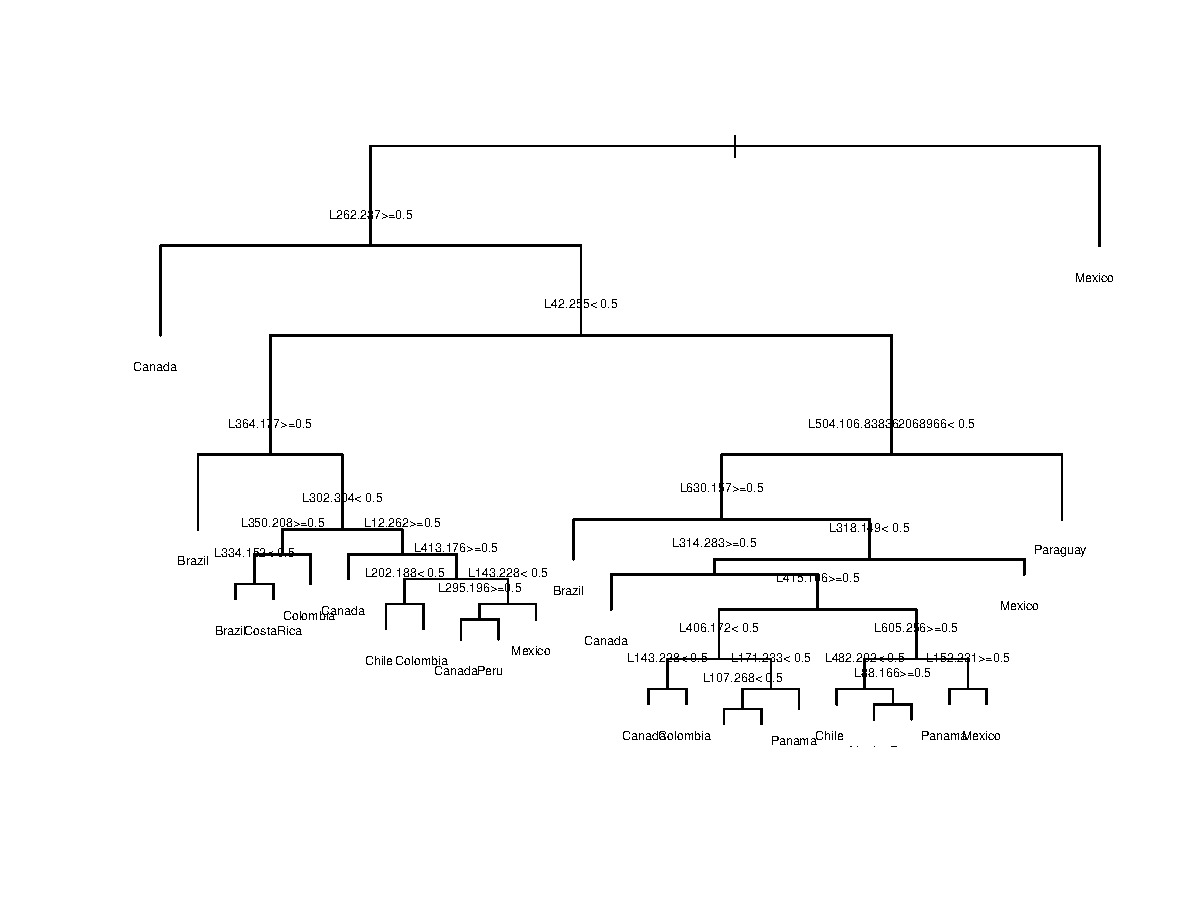
\includegraphics[scale=0.6]{figures/tree.pdf}
		\caption{Arbre de classification obtenu après scindage.}
		\label{fig:prune_tree}
	\end{center}
\end{figure}
Comme on peut le voir sur la figure \ref{fig:prune_tree}, on obtient un arbre plus petit. Aussi seules 5 variables sont utilisées dans sa construction. On obtient un taux d'erreur pire que précédemment.\vspace{2mm}
\begin{lstlisting}
	preds.prune = predict(prun, newdata = NAm2[-train,-c(1:3,5:8)], type = "class")
	mean(NAm2$Country[-train] != preds.prune)
	## [1] 0.5212766
\end{lstlisting}
Il n'est pas étonnant d'obtenir des taux moins bons. En fait, nous somme limités dans la taille de notre arbre d'une part par le package que nous utilisons et d'autre part par notre faible nombre d'observations. Ce qui entraîne qu'un faible nombre de variables soient utilisées dans la construction de l'arbre.
\subsubsection{Bagging}
Nous essayons maintenant avec la méthode \textit{bagging}.\vspace{2mm}
\begin{lstlisting}
	require(randomForest)
	set.seed(12345)
	mtry = ncol(NAm2) - 8
	fit.bag = randomForest(Country~., data=NAm2[,-c(1:3,5:8)], subset = train, mtry=mtry, importance=T)
	preds.bag = predict(fit.bag, newdata = NAm2[-train,-c(1:3,5:8)], type = "class")
	mean(NAm2$Country[-train] != preds.bag)
	## [1] 0.3191489
\end{lstlisting}
On note une amélioration par rapport à l'arbre de classification puisque le taux d'erreur descend à 0.32. Mais il demeure très élevé comparé à la régression logistique ou encore au KNN.
\subsubsection{Random Forests}
Enfin nous appliquons la méthode random forests. Elle est identique au bagging sauf que plutôt que de considérer toutes les variables à chaque coupe, on considère un sous-ensemble de $m$ variables. On teste d'abord le cas classique $m=\sqrt{p} = 75$.\vspace{2mm}
\begin{lstlisting}
	set.seed(12345)
	fit.rand = randomForest(Country~., data=NAm2[,-c(1:3,5:8)], subset = train, mtry=75)
	preds.rand = predict(fit.bag, newdata = NAm2[-train,-c(1:3,5:8)], type = "class")
	mean(NAm2$Country[-train] != preds.rand)
	## [1] 0.3191489
\end{lstlisting}
Bizarrement on obtient le même taux d'erreur que le bagging. Nous avons testé
d'autres valeurs pour $m$ et nous obtenons toujours le même taux d'erreur. Il
apparaît donc qu'il s'agit du meilleur taux que l'on peut espérer avec cette
méthode. \\
Cependant on se demande si le fait qu'il y ait trop de prédicteurs ne nuit pas
à la méthode. C'est à dire que l'arbre pourrait atteindre un des critères d'arrêt
alors qu'il ne considère qu'une faible partie des variables et que celles-ci ne
sont pas assez complètes. \\
Nous décidons de tester la méthode en utilisant les axes principaux obtenus avec 
l'ACP afin de contruire l'arbre. Nous procédons une nouvelle fois par validation
croisée afin de choisir le meilleur nombre de composantes. Nous trouvons qu'il 
faut prendre les 40 premières composantes. L'erreur test ensuite obtenue par le
modèle est de 0.180. C'est donc meilleur que de prendre toutes les données. A 
part la justification précédente il faudra connaître un peu plus en détail le
code utilisé par randomForest pour expliquer cette tendance. \\
Voici le code utilisé pour obtenir le résultat:

\begin{lstlisting}
#Recherche du meilleur nombre de composantes
err.cv = numeric(40)
i=1
for (numComp in seq(10, 400, 10)) {
	print(i)
	err = numeric(10)
	for (k in 0:9) {
		entr=c((1+k*40):((k+1)*40))
		fit.bag = randomForest(Country~., data=NA.pca.train[-entr,1:(numComp+1)], 
					mtry=round(sqrt(numComp)), importance=T)
		preds.bag = predict(fit.bag, newdata = NA.pca.train[entr,1:(numComp+1)], 
					type = "class")
		err[k+1] = mean(NA.pca.train$Country[entr] != preds.bag)
	}
	err.cv[i]=mean(err)
	i=i+1
}
#Calcul de l'erreur test
fit.bag = randomForest(Country~., data=NA.pca.train[,1:41],
			mtry=round(sqrt(40)), importance=T)
test_data = scale(NAm2[-train,-c(1:8)], NA.comp$center, NA.comp$scale) %*% NA.comp$rotation
test.log = as.data.frame(test_data[,1:40])
preds.bag = predict(fit.bag, newdata = test.log, type = "class")
mean(NA.pca.train$Country[] != preds.bag)
\end{lstlisting}


\section{Conclusion}
Le tableau ci-contre récapitule les différentes méthodes essayées ainsi que leur taux d'erreur. \vspace{-4mm}
\begin{center}
	\captionof{table}{Taux d'erreur des différentes méthodes}
	\begin{tabular}{|c|c|}
		\hline
		Méthode & Taux d'erreur \\ \hline
		ACP + logistique & 0.106 \\ \hline
		ACP + LDA & 0.096 \\ \hline
		Logistique + Ridge & 0.053 \\ \hline
		Logistique + Lasso & 0.138 \\ \hline
		KNN & 0.149 \\ \hline
		Arbre de classification & 0.489 \\ \hline
		Pruning & 0.52 \\ \hline
		Random forest & 0.32 \\ \hline
		ACP + Random forest & 0.180 \\ \hline
	\end{tabular}
	\label{tab:resume}
\end{center}
~\\
La régression logistique avec une régularisation Ridge est clairement la
meilleure. En effet elle donne le taux d'erreur le plus faible. Elle se trompe
sur 5 individus dont 4 appartiennent à la classe \textit{Péru} qui n'avait que
10 individus dans l'ensemble d'apprentissage. Il est tout à fait raisonnable de
dire qu'avec plus d'effectifs dans cette classe, nous obtiendrons un meilleur
taux d'erreur.\vspace{3mm}\\

Les données semblent linéairement séparables puisque l'analyse discriminante et
la régression logistique sont les méthodes qui donnent les meilleurs
résultats.\\

Les méthodes basées sur les arbres de décision marchent assez mal ici car il
n'est pas possible de construire des arbres suffisamment grand. On a
également essayer d'utiliser les composantes principales pour construire les
arbres. Le taux d'erreur diminue assez fortement mais pas assez cependant
pour que cette méthode soit intéréssante. \\
La régression logistique avec Ridge quant à elle a très bien marchée.
\vspace{3mm}\\

En somme, nous voyons qu'il est possible en fonction des marqueurs génétiques
d'associer un individu à un pays donné. Il est tout à fait raisonnable
d'affirmer qu'avec un nombre d'observations plus importants, nous obtiendrons
des résultats tout à fait similaires si nous choisissons d'effectuer la
classification en fonction de la population plutôt que du pays.

\end{document}
